% This is samplepaper.tex, a sample chapter demonstrating the
% LLNCS macro package for Springer Computer Science proceedings;
% Version 2.20 of 2017/10/04
%
\documentclass[runningheads]{llncs}
%
\usepackage{graphicx}
\usepackage{amssymb}
\usepackage{amsmath}
\usepackage{hyperref}

% Used for displaying a sample figure. If possible, figure files should
% be included in EPS format.
%
% If you use the hyperref package, please uncomment the following line
% to display URLs in blue roman font according to Springer's eBook style:
% \renewcommand\UrlFont{\color{blue}\rmfamily}

\begin{document}
%
\title{Contribution Title\thanks{Supported by organization x.}}
%
%\titlerunning{Abbreviated pa`per title}
% If the paper title is too long for the running head, you can set
% an abbreviated paper title here
%
\author{First Author\inst{1}\orcidID{0000-1111-2222-3333} \and
Second Author\inst{2,3}\orcidID{1111-2222-3333-4444} \and
Third Author\inst{3}\orcidID{2222--3333-4444-5555}}
%
\authorrunning{F. Author et al.}
% First names are abbreviated in the running head.
% If there are more than two authors, 'et al.' is used.
%
\institute{Princeton University, Princeton NJ 08544, USA \and
Springer Heidelberg, Tiergartenstr. 17, 69121 Heidelberg, Germany
\email{lncs@springer.com}\\
\url{http://www.springer.com/gp/computer-science/lncs} \and
ABC Institute, Rupert-Karls-University Heidelberg, Heidelberg, Germany\\
\email{\{abc,lncs\}@uni-heidelberg.de}}
%
\maketitle              % typeset the header of the contribution
%
\begin{abstract}
The abstract should briefly summarize the contents of the paper in
150--250 words.

\keywords{First keyword  \and Second keyword \and Another keyword.}
\end{abstract}
%
%
%
\section{Problem Specification}
\begin{enumerate}
    \item \textbf{State:} For \( k \in \{3, 4, 5\} \),  A \( k \times k \) matrix \( M \) with each entry \( m_{i, j} \) being a unique integer from \( \{0, 1, \cdots, 8 \} \) where 0 represents the blank tile.
    \item \textbf{Initial State:} Puzzle can start in any state \textit{s}.
    \item \textbf{Actions or \textit{Actions(s)}:} Actions refer to the movements of the blank tile \( m_{k, l} \) \textit{Left, Right, Up, or Down}. More formally ...
    % Q: An action swaps the tile \( m_{k, l} \) with the tile \(\{ m_{i,j} \in M: (i=k+1, j=l) \vee (i=k, j=l+1) \vee (i=k-1, j=l) \vee (i=k, j=l-1) \}\)
    \item \textbf{Transition Model or \textit{Result(s,a)}:} \( Result(s, a) \) swaps the pair of tiles specified in action \( a \) in the current state \textit{s} and returns this new state \textit{s'}.
    \item \textbf{Goal State:} TODO: insert picture of goal state
    \item \textbf{Path Cost:} Every step cost \textit{c(s, a, s') = 1}, and the path cost is the summation of the step costs from the initial state to the goal state.
\end{enumerate}

\section{Technical Analysis of the Selected Algorithms and Heuristics}
\begin{enumerate}
    \item \textbf{nodes:} state \textit{s}
    \item \textbf{edges:} \textit{Result(s, a)}, which has a step cost of 1
\end{enumerate}

% TODO: Update unsolvable rule to k-puzzle 
\subsection{Rule to Check if a 8 puzzle is Solvable}
It is not possible to solve an instance of 8 puzzle if number of inversions is odd in the input state. 
Inversion is defined as a pair of tiles form an inversion if the values on tiles are in reverse order of their appearance in goal state. Source \href{https://www.geeksforgeeks.org/check-instance-8-puzzle-solvable/}{here}.

\subsection{Uninformed Search}
% TODO: Update report of Uninformed search from BFS to IDS
% TODO: IDS implementation
\begin{enumerate}
    \item \textbf{Implementation:} Graph-based IDS. Step costs are equal, thus it is optimal. Furthermore, since the search space is large and the depth of the solution is not known, IDS is preferred. (P90)
    \item \textbf{Correctness:} IDS is complete (ie it will find a solution if it exists and \textit{b} is finite (ie \( b \leq 4 \)), thus it is correct.
    \item \textbf{Complexity:} \( O(d) \)
\end{enumerate}

% TODO: A* Implementation
% TODO: Implementation of 3 heuristics
% TODO: Prove consistency of heuristics
% Q: Need to prove complexity and correctness of algos?

\subsection{Informed Search}
\begin{enumerate}
    \item \textbf{Implementation:} \( A^* \) search. It improves on greedy best first search (ie \( f(n) = h(n) \)) as it avoids expanding paths that are already expensive (ie \( f(n) = g(n) + h(n) \)).
    \item \textbf{Tree or graph?:} Tree search. By Lemma 1, if \( h(n) \) is consistent, then the values of \( f(n) \) along any path are nondecreasing. Thus it does not matter if we add the explored node back into our frontier: there will exist another node \( n' \) such that \( f(n') < f(n) \).
    \item \textbf{Correctness:} \( A^* \) search is complete (ie it will find a solution if it exists and there is a finite no. of nodes with \( f(n) \leq C^{*} \), where \( C^* \) is the cost of the optimal solution path.
    \item \textbf{Complexity:} \( O(b^{h^*(s_0) - h(s_0)}) \) 
\end{enumerate}

\subsection{Manhattan Distance} 
To prove that Manhattan Distance is consistent.
\begin{proof} Proof by Cases
    \begin{enumerate}
        \item \( |h(n') - h(n) = 1| \) (\( \because c(n, a, n') = 1 \), any node n' is 1 step away from node n)
        \item Case 1: \( h(n') = h(n) + 1 \)
        \begin{enumerate}
            \item \( h(n) \leq h(n) + 1 + 1 \implies h(n) \leq h(n') + c(n, a, n') \)
        \end{enumerate}
        \item Case 2: \( h(n') = h(n) - 1 \)
        \begin{enumerate}
            \item \( h(n) \leq h(n) - 1 + 1 \implies h(n) \leq h(n') + c(n, a, n') \)
        \end{enumerate}
        \item For both cases of \( h(n') \), \( h(n) \) is consistent. (\(\bullet\))
    \end{enumerate}
\end{proof}

\subsection{Euclidean Distance}

\subsection{Number of tiles out of row + Number of tiles out of column} 
\textbf{Relaxed Problem.} A tile can move anywhere within the row or column. This guarantees admissibility. \\
TODO: Prove consistency (?). However, since both hamming and manhatten distance are consistent as shown \href{https://www.cs.princeton.edu/courses/archive/fall12/cos226/checklist/8puzzle.html}(here), 
it's likely that this variant of hamming distance will be consistent too.

% Q: Ask if this heuristic is non trivial.
\subsection{Linear conflict + Manhattan Distance}
Add two to the Manhattan priority function whenever two tiles are in their goal row (or column) but are reversed relative to their goal position. Paper available \href{https://cse.sc.edu/~mgv/csce580sp15/gradPres/HanssonMayerYung1992.pdf}(here).\\
This is likely to be consistent since it is a linear transformation of the manhattan distance. \\ 

\section{Experimental Setup}
\begin{enumerate}
    \item \textbf{Number of Nodes Generated:} Time Complexity
    \item \textbf{Size of Frontier:} Space Complexity
    \item Plot puzzle difficulty or multiple iterations for the same puzzle difficulty against time/space complexity 
\end{enumerate}

\section{First Section}
\subsection{A Subsection Sample}
Please note that the first paragraph of a section or subsection is
not indented. The first paragraph that follows a table, figure,
equation etc. does not need an indent, either.

Subsequent paragraphs, however, are indented.

\subsubsection{Sample Heading (Third Level)} Only two levels of
headings should be numbered. Lower level headings remain unnumbered;
they are formatted as run-in headings.

\paragraph{Sample Heading (Fourth Level)}
The contribution should contain no more than four levels of
headings. Table~\ref{tab1} gives a summary of all heading levels.

\begin{table}
\caption{Table captions should be placed above the
tables.}\label{tab1}
\begin{tabular}{|l|l|l|}
\hline
Heading level &  Example & Font size and style\\
\hline
Title (centered) &  {\Large\bfseries Lecture Notes} & 14 point, bold\\
1st-level heading &  {\large\bfseries 1 Introduction} & 12 point, bold\\
2nd-level heading & {\bfseries 2.1 Printing Area} & 10 point, bold\\
3rd-level heading & {\bfseries Run-in Heading in Bold.} Text follows & 10 point, bold\\
4th-level heading & {\itshape Lowest Level Heading.} Text follows & 10 point, italic\\
\hline
\end{tabular}
\end{table}


\noindent Displayed equations are centered and set on a separate
line.
\begin{equation}
x + y = z
\end{equation}
Please try to avoid rasterized images for line-art diagrams and
schemas. Whenever possible, use vector graphics instead (see
Fig.~\ref{fig1}).

\begin{figure}
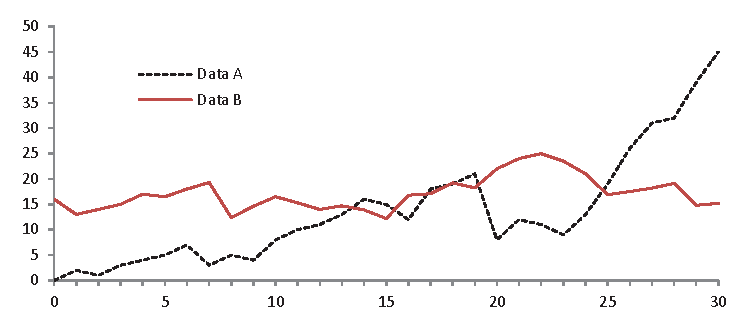
\includegraphics[width=\textwidth]{fig1.eps}
\caption{A figure caption is always placed below the illustration.
Please note that short captions are centered, while long ones are
justified by the macro package automatically.} \label{fig1}
\end{figure}

\begin{theorem}
This is a sample theorem. The run-in heading is set in bold, while
the following text appears in italics. Definitions, lemmas,
propositions, and corollaries are styled the same way.
\end{theorem}
%
% the environments 'definition', 'lemma', 'proposition', 'corollary',
% 'remark', and 'example' are defined in the LLNCS documentclass as well.
%
\begin{proof}
Proofs, examples, and remarks have the initial word in italics,
while the following text appears in normal font.
\end{proof}
For citations of references, we prefer the use of square brackets
and consecutive numbers. Citations using labels or the author/year
convention are also acceptable. The following bibliography provides
a sample reference list with entries for journal
articles~\cite{ref_article1}, an LNCS chapter~\cite{ref_lncs1}, a
book~\cite{ref_book1}, proceedings without editors~\cite{ref_proc1},
and a homepage~\cite{ref_url1}. Multiple citations are grouped
\cite{ref_article1,ref_lncs1,ref_book1},
\cite{ref_article1,ref_book1,ref_proc1,ref_url1}.
%
% ---- Bibliography ----
%
% BibTeX users should specify bibliography style 'splncs04'.
% References will then be sorted and formatted in the correct style.
%
% \bibliographystyle{splncs04}
% \bibliography{mybibliography}
%
\begin{thebibliography}{8}
\bibitem{ref_article1}
Author, F.: Article title. Journal \textbf{2}(5), 99--110 (2016)

\bibitem{ref_lncs1}
Author, F., Author, S.: Title of a proceedings paper. In: Editor,
F., Editor, S. (eds.) CONFERENCE 2016, LNCS, vol. 9999, pp. 1--13.
Springer, Heidelberg (2016). \doi{10.10007/1234567890}

\bibitem{ref_book1}
Author, F., Author, S., Author, T.: Book title. 2nd edn. Publisher,
Location (1999)

\bibitem{ref_proc1}
Author, A.-B.: Contribution title. In: 9th International Proceedings
on Proceedings, pp. 1--2. Publisher, Location (2010)

\bibitem{ref_url1}
LNCS Homepage, \url{http://www.springer.com/lncs}. Last accessed 4
Oct 2017
\end{thebibliography}
\end{document}
